\chapter{Fundamentação Teórica}
\label{cap:fundamentacao-teorica}

Este capítulo apresenta os conceitos, métodos e abordagens científicas que embasam a análise do método USARP e a estratégia empírica adotada. Inicialmente, discute-se o papel da usabilidade na Engenharia de Software e sua relação com a qualidade de sistemas interativos. Em seguida, aborda-se a Engenharia de Requisitos com ênfase na elicitação de requisitos de usabilidade. Posteriormente, o método USARP é detalhado de forma aprofundada, incluindo seus fundamentos conceituais, estrutura operacional e evolução. Em seguida, apresenta-se o \textit{Technology Acceptance Model} (TAM), base do instrumento de avaliação empregado nos estudos analisados. Por fim, são discutidos os fundamentos da síntese de evidências empíricas em Engenharia de Software, da análise temática e da Análise de Componentes Principais (PCA), técnicas utilizadas para a síntese e a interpretação dos dados deste estudo.

\section{Usabilidade na Engenharia de Software}

A usabilidade é reconhecida como um atributo central da qualidade de software, especialmente em sistemas interativos. De acordo com a norma ISO/IEC 25010, a usabilidade refere-se ao grau em que um sistema pode ser utilizado por usuários específicos para atingir objetivos definidos com eficácia, eficiência e satisfação, considerando um contexto de uso específico \cite{iso25010}. Essa definição evidencia que a usabilidade não se restringe à interface gráfica, mas envolve aspectos relacionados ao comportamento do sistema, às funcionalidades disponibilizadas e à forma como o usuário interage com essas funcionalidades ao longo do tempo.

Na Engenharia de Software, a usabilidade passou a ser compreendida como um fator estratégico para o sucesso de produtos digitais. Estudos clássicos demonstram que sistemas com baixa usabilidade tendem a apresentar maior taxa de erros operacionais, baixa aceitação por parte dos usuários e aumento nos custos de suporte e manutenção \cite{nielsen1993}. Além disso, decisões de projeto tomadas nas fases iniciais do desenvolvimento exercem influência direta sobre a experiência do usuário e sobre a sustentabilidade do sistema ao longo de seu ciclo de vida \cite{preece2015}.

Apesar desse reconhecimento, a usabilidade ainda é frequentemente tratada de forma tardia no processo de desenvolvimento, sendo avaliada apenas em fases finais, geralmente associadas a testes de interface ou validação com usuários. Essa abordagem corretiva limita a capacidade de resolver problemas estruturais de uso, uma vez que ajustes realizados após a implementação tendem a demandar maior esforço, custo e retrabalho \cite{juristo2007}.

\section{Engenharia de Requisitos e Requisitos de Usabilidade}

A Engenharia de Requisitos compreende um conjunto de atividades voltadas à identificação, análise, documentação e gerenciamento dos requisitos de um sistema, com o objetivo de garantir que o software atenda às necessidades reais de seus usuários e demais stakeholders \cite{sommerville2011}. Tradicionalmente, os requisitos são classificados em funcionais e não funcionais. Os requisitos de usabilidade são, em geral, enquadrados como requisitos não funcionais; contudo, essa classificação tem se mostrado insuficiente para representar adequadamente seu impacto no sistema.

Requisitos de usabilidade apresentam características particulares que dificultam sua elicitação e especificação. Eles são frequentemente subjetivos, dependentes do contexto de uso e fortemente influenciados por fatores humanos, como expectativas, experiência prévia e limitações cognitivas dos usuários \cite{ardito2014}. Além disso, muitos aspectos de usabilidade manifestam-se por meio de comportamentos funcionais do sistema, afetando diretamente o design e a arquitetura do software.

Nesse contexto, Juristo, Moreno e Sánchez-Segura propuseram o conceito de \textit{Functional Usability Features} (FUFs), defendendo que determinados aspectos de usabilidade devem ser tratados como funcionalidades explícitas do sistema \cite{juristo2007}. As FUFs são decompostas em mecanismos de usabilidade, como feedback, prevenção de erros, alertas, desfazer ações e ajuda multinível, que podem ser especificados como requisitos verificáveis e rastreáveis. Essa abordagem reforça a necessidade de considerar a usabilidade desde a fase de elicitação de requisitos, integrando-a às decisões técnicas e funcionais do sistema.

\section{O Método USARP}

O método USARP (\textit{Usability Requirements with Personas and User Stories}) foi proposto com o objetivo de apoiar a elicitação e a especificação sistemática de requisitos de usabilidade em fases iniciais do desenvolvimento de software, especialmente em contextos ágeis \cite{oliveirajr2020}. O método surge da constatação de que, embora existam diretrizes e recomendações de usabilidade bem estabelecidas, há uma lacuna prática quanto à sua incorporação efetiva durante a elicitação de requisitos, sobretudo por equipes não especialistas em usabilidade.

O USARP fundamenta-se na integração de três elementos principais: \textit{personas}, \textit{user stories} e mecanismos de usabilidade derivados das \textit{Functional Usability Features}. As \textit{personas} são utilizadas para representar perfis de usuários reais, considerando suas características, necessidades, objetivos e limitações. As \textit{user stories} oferecem um formato simples e amplamente adotado no desenvolvimento ágil para a especificação de requisitos sob a perspectiva do usuário. Os mecanismos de usabilidade atuam como guias estruturados que direcionam a reflexão sobre aspectos funcionais relacionados à qualidade de uso. Na Figura~\ref{fig:cartas-mecanismos-usarp}, são apresentadas as cartas de mecanismos de usabilidade do USARP, que orientam a reflexão sobre funcionalidades relacionadas à qualidade de uso. Já as cartas de requisitos de usabilidade, ilustradas na  Figura~\ref{fig:cartas-requisitos-usarp}, auxiliam na especificação desses requisitos. Por fim, a Figura~\ref{fig:cartas-prototipação-usarp} traz as cartas de prototipação, que apoiam a materialização das soluções propostas.

\begin{figure}[h!]
    \centering
    \caption{Exemplos de cartas de mecanismos de usabilidade do método USARP}
    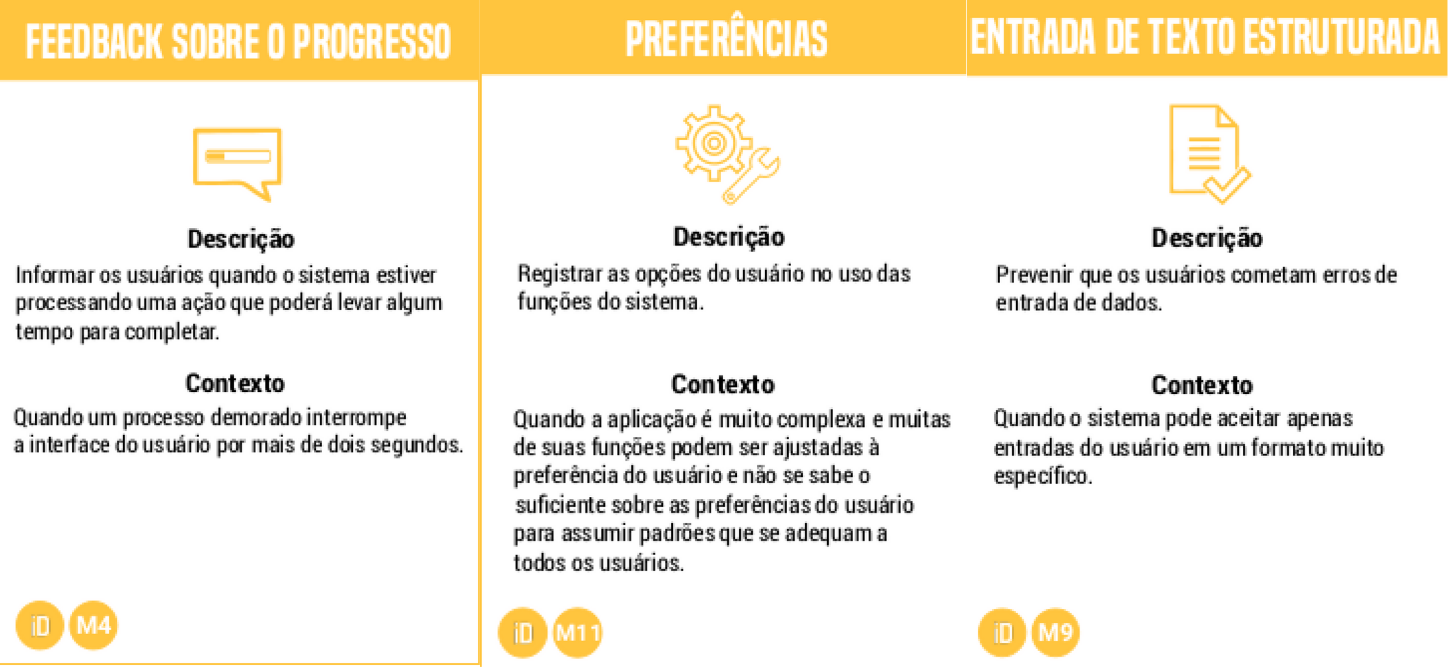
\includegraphics[width=0.9\textwidth]{figuras/cartas_mecanismos.png}
    \label{fig:cartas-mecanismos-usarp}
    \Fonte{Elaborado pelo autor (2025), com base em Oliveira, Ferreira e Marques (2020).}
\end{figure}
\begin{figure}[h!]
    \centering
    \caption{Exemplos de cartas de requisitos de usabilidade do método USARP}
    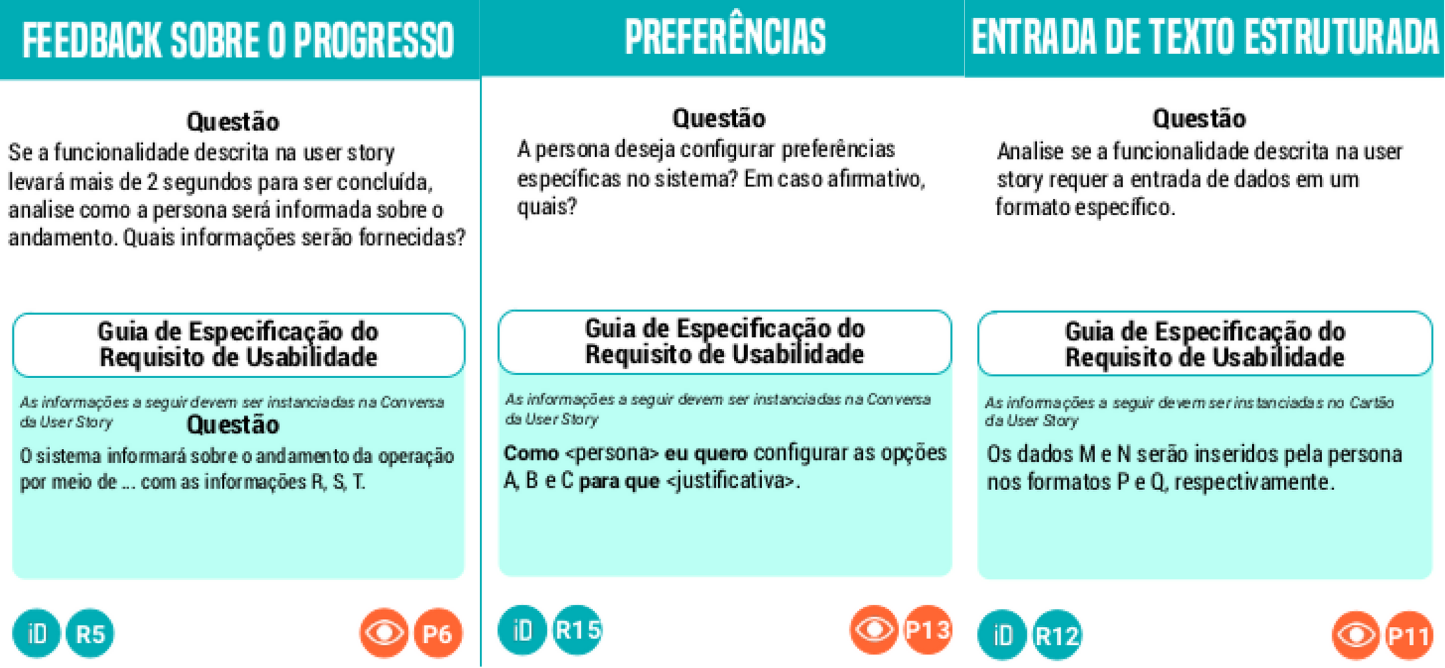
\includegraphics[width=0.9\textwidth]{figuras/cartas_requisitos.png}
    \label{fig:cartas-requisitos-usarp}
    \Fonte{Elaborado pelo autor (2025), com base em Oliveira, Ferreira e Marques (2020).}
\end{figure}
\begin{figure}[h!]
    \centering
    \caption{Exemplos de cartas de prototipação do método USARP}
    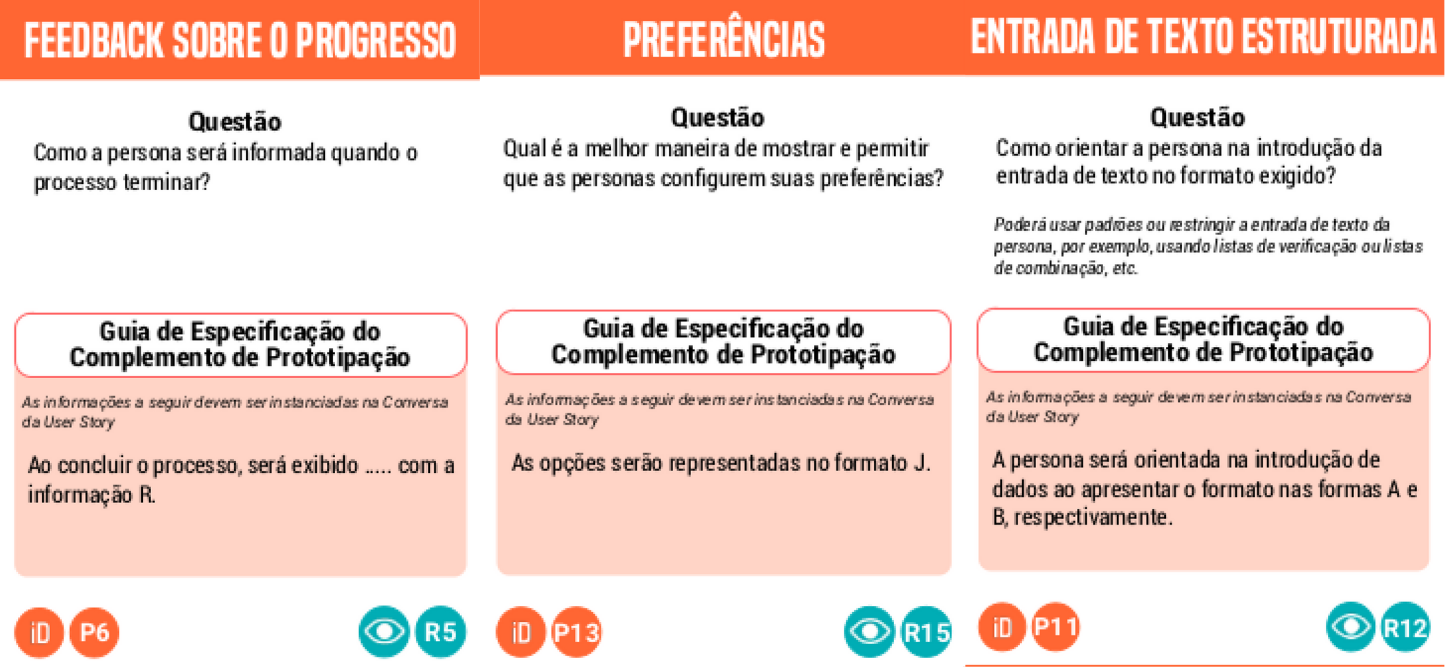
\includegraphics[width=0.9\textwidth]{figuras/cartas_prototipação.png}
    \label{fig:cartas-prototipação-usarp}
    \Fonte{Elaborado pelo autor (2025), com base em Oliveira, Ferreira e Marques (2020).}
\end{figure}

\FloatBarrier

O método propõe um processo estruturado que se inicia com a criação de \textit{personas}, segue pela extração de requisitos potenciais e culmina na escrita e no enriquecimento de \textit{user stories} com mecanismos de usabilidade explícitos. Essa abordagem permite que aspectos de usabilidade sejam discutidos, negociados e documentados de forma sistemática, reduzindo a dependência de especialistas e promovendo maior conscientização da equipe de desenvolvimento.

Estudos empíricos indicam que o USARP é eficaz na obtenção de requisitos de usabilidade, embora também evidenciem desafios relacionados à carga cognitiva imposta por alguns mecanismos e à necessidade de maior direcionamento no uso dos artefatos \cite{marques2022}. Esses resultados motivaram a evolução do método, incluindo a transformação dos mecanismos de usabilidade em cartas, com o objetivo de tornar o processo mais dinâmico, acessível e colaborativo.

Mais recentemente, \citeonline{marquesfiori2023} consolidaram uma evolução do método a partir de um estudo exploratório conduzido em uma turma de Engenharia de Software, no qual foram observadas dificuldades na seleção das cartas durante as sessões de \textit{brainstorming}. Com base nessa análise, os autores revisaram as cartas, removendo conteúdos redundantes e combinando cartas de conteúdo semelhante, com a eliminação de oito cartas. Além disso, propuseram dois novos artefatos: um \textit{checklist} que organiza os mecanismos de usabilidade em quatro categorias (personalização do sistema, feedback do sistema, controle e apoio ao usuário e entrada de dados) e um quadro para dispor as cartas selecionadas conforme as características dos usuários e do sistema. O processo de adoção do método foi atualizado para incorporar duas novas etapas, de seleção e de organização das cartas, anteriores ao \textit{brainstorming}. É essa versão evoluída, baseada em cartas e em uma etapa de filtragem por \textit{checklist}, que fundamenta os estudos de aplicação analisados neste trabalho.

\section{O Modelo de Aceitação de Tecnologia (TAM)}

O instrumento quantitativo utilizado nos estudos primários analisados fundamenta-se no \textit{Technology Acceptance Model} (TAM), modelo proposto por \citeonline{davis1989} para explicar a aceitação e o uso de tecnologias da informação. O TAM postula que a intenção de uso de uma tecnologia é determinada, sobretudo, por dois construtos: a utilidade percebida (\textit{perceived usefulness}), definida como o grau em que uma pessoa acredita que o uso de determinado sistema melhoraria seu desempenho, e a facilidade de uso percebida (\textit{perceived ease of use}), entendida como o grau em que a pessoa acredita que esse uso seria livre de esforço \cite{davis1989}. Esses construtos têm sido amplamente empregados para avaliar a aceitação de métodos, técnicas e ferramentas no campo da Engenharia de Software.

Em sua evolução, o modelo foi estendido pelo TAM3, que detalha os determinantes da utilidade e da facilidade de uso percebidas e organiza um conjunto de intervenções capazes de influenciar a aceitação de uma tecnologia ao longo de sua adoção \cite{venkatesh2008}. No contexto deste trabalho, o TAM oferece o arcabouço conceitual para o bloco de percepção geral do instrumento, cujos itens relativos a utilidade, produtividade, eficácia e facilidade de aplicação do método derivam diretamente dos construtos de utilidade e de facilidade de uso percebidas.

\section{Síntese de Evidências Empíricas em Engenharia de Software}

A consolidação de evidências provenientes de múltiplos estudos é uma estratégia central da Engenharia de Software Empírica, sobretudo em cenários caracterizados por heterogeneidade de contextos e de métodos \cite{kitchenham2009}. Revisões sistemáticas e estudos de síntese permitem identificar, avaliar criticamente e integrar resultados de estudos primários por meio de procedimentos explícitos e reprodutíveis, reduzindo vieses e aumentando a confiabilidade das conclusões \cite{kitchenham2009,kitchenham2007}.

A literatura distingue, contudo, diferentes graus e formas de síntese. A meta-análise, em sentido estrito, consiste na agregação estatística de tamanhos de efeito padronizados provenientes de estudos comparáveis, usualmente com grupos de comparação e com a estimação da heterogeneidade entre estudos \cite{rodrigues2010}. Em grande parte da pesquisa em Engenharia de Software, entretanto, essa agregação não é viável, seja pela ausência de grupos de controle, seja pela diversidade de instrumentos e de desenhos de estudo. Por essa razão, \citeonline{cruzesdyba2010} observam que muitas revisões da área não realizam síntese estatística propriamente dita e defendem a adoção de métodos de síntese mais amplos, como as sínteses narrativas e temáticas, capazes de integrar evidências qualitativas e quantitativas de naturezas distintas.

É nesse espectro que se situa o presente trabalho. Não se trata de uma meta-análise, pois não há agregação ponderada de tamanhos de efeito nem grupo de comparação controlado; trata-se de uma síntese empírica que consolida, no nível do respondente, os dados de levantamento de diferentes aplicações de um mesmo método e os integra a uma síntese qualitativa das evidências reportadas. Essa abordagem é adequada para investigar padrões de percepção, uso e avaliação de um método de Engenharia de Software aplicado em diferentes contextos acadêmicos e industriais, em linha com a discussão de \citeonline{runeson2012} sobre estudos de caso conduzidos em múltiplos ambientes, nos quais a comparação entre cenários distintos fortalece a validade externa dos resultados e aprofunda a compreensão das condições de uso de um método.

\section{Análise Temática e Síntese Qualitativa}

A interpretação das evidências qualitativas deste trabalho apoia-se na análise temática, abordagem voltada à identificação, à organização e à interpretação de padrões de significado, denominados temas, em dados textuais \cite{braunclarke2006}. A análise temática é particularmente adequada para sintetizar respostas abertas e relatos de experiência, por admitir tanto a codificação indutiva, derivada dos próprios dados, quanto o diálogo com categorias previamente reportadas na literatura \cite{saldana2013}. No campo da Engenharia de Software, a síntese qualitativa e temática é reconhecida como um recurso essencial para integrar evidências provenientes de estudos conduzidos em contextos distintos \cite{cruzesdyba2010}. Neste estudo, a análise temática é aplicada às respostas abertas consolidadas e articulada às codificações originais dos estudos primários, conforme detalhado na metodologia.

\section{Análise de Componentes Principais}

A Análise de Componentes Principais (PCA) é uma técnica estatística multivariada de redução de dimensionalidade que transforma um conjunto de variáveis correlacionadas em um número menor de variáveis não correlacionadas, denominadas componentes principais, que retêm a maior parte da variância original dos dados \cite{jolliffe2002}. Cada componente é uma combinação linear das variáveis observadas, e a análise das cargas associadas a cada componente permite interpretar as estruturas latentes que organizam as respostas \cite{hair2019}. Na presente síntese, a PCA é empregada de forma exploratória e descritiva, com o objetivo de resumir a variabilidade das avaliações e identificar agrupamentos de itens, e não como análise fatorial confirmatória, ressalva detalhada na metodologia em razão das características dos dados, em especial o tamanho reduzido da amostra e o acentuado efeito de teto.